\chapter{Forme differenziali}
Si passi ora alla trattazione delle forme differenziali.
Per fare ciò, si consideri $A \subseteq \mathbb{R}^n$ aperto. Siano poi $a_1(x), \dots, a_n(x)$ con $x \in A$ funzioni continue in $A$ e siano $dx_1, \dots, dx_n$ funzioni lineari da $\R^n$ a $\R$ tali che $h \mapsto h_i$.
\begin{definition} \label{Def: Forma differenziale}
Si dice \textbf{forma differenziale} un'applicazione $\omega:\ x \in A \to  (\mathbb{R}^n)^*$, cioè il duale di $\mathbb{R}^n$, data dall'espressione:
\begin{equation}
    \omega= \omega(x)= \sum\limits_{i=1}^{n}{a_i(x)dx_i}
\end{equation}
con $a_i$ detti \textbf{coefficienti} della forma differenziale $\omega$.
\end{definition}
\begin{oss}
    Se $h$ è un vettore generico di $\R^n$, il valore assunto da $\omega(x)$ in $h$ è dato da:
    \begin{equation}
        \omega(x)(h)=\sum\limits_{i=1}^{n}{a_i(x)dx_i(h)}= \sum\limits_{i=1}^{n}{a_i(x)h_i}
    \end{equation}
\end{oss}
\begin{oss}
A tal proposito, si dice \textit{campo vettoriale} associato la funzione $F: A\subseteq \R^n \to \R^n$ data da
\begin{equation}
    F=F(x)=(a_1(x), \dots, a_n(x_n))
\end{equation}
Inoltre, si può notare che il legame tra i due è dato da:
\begin{equation} \label{Eq: Campo vettoriale}
    \omega(x)= \langle F(x), dx \rangle
\end{equation}
dove $dx= (dx_1,\dots, dx_n)$.
\end{oss}
\begin{oss}
Presa $f$ differenziabile in $A$, si può osservare che il suo differenziale $df$ sarà dato da
\begin{equation} \label{Eq: Differenziale}
    df(x)= \sum\limits_{i=1}^{n}{\frac{\partial f}{\partial x_i}(x)\ dx_i}= \langle \nabla f(x), dx\rangle
\end{equation}
\end{oss}
\section{Integrale curvilineo di seconda specie}
\begin{definition} \label{Def: Integrale curvilineo di seconda specie}
    Sia $A \subseteq \R$ e sia $\omega: A \to (\R)^*$ con coefficienti continui. Sia inoltre $\gamma$ una curva regolare di parametrizzazione $\varphi: [a, b] \to A$. Allora si definisce \textbf{integrale curvilineo di seconda specie} o integrale di $\omega$ lungo $\gamma$ la quantità:
    \begin{equation} \label{Eq: Integrale curvilineo di seconda specie}
        \int\limits_\gamma \omega := \int\limits_{a}^{b}\left( \sum\limits_{i=1}^{n}{a_i(\varphi(t))\ \varphi_i'(t)}\right)\, dt
    \end{equation}
\end{definition}
Per tale ragione, si può osservare che l'integrale curvilineo di seconda specie di un campo vettoriale $F$ associato ad una forma differenziale $\omega$ lungo una curva $\gamma$ è dato dall'integrale curvilineo di prima specie di 
\begin{equation}
    \int\limits_{\gamma}{\langle F, T \rangle}\, ds
\end{equation}
e in particolare vale:
\begin{equation}
    \int\limits_{\gamma}{\omega}= \int\limits_{a}^{b} {\langle F(\gamma(t)), \gamma'(t)\rangle}\, dt = \int\limits_{a}^{b} {\langle F(\gamma(t)), T(\gamma(t))\rangle} |\gamma'(t)|\, dt = \int\limits_{\gamma}{\langle F, T \rangle}\, ds
\end{equation}
Inoltre, vale il seguente risultato.
\begin{theorem}[Invarianza per equivalenza di curve] \label{Teo: Invarianza per equivalenza di curve dell'integrale curv di 2 specie}
    Siano $\gamma,\ , \gamma'$ due curve equivalenti e sia $\omega$ una forma differenziale definita in $A$. Allora
    \begin{equation}
        \int\limits_\gamma { \omega} = \int\limits_{\gamma'}{\omega}\quad \text{oppure} \quad \int\limits_\gamma { \omega} = -\int\limits_{\gamma'}{\omega}
    \end{equation}
    se sono percorse nello stesso verso o in verso opposto, rispettivamente.
\end{theorem}
\begin{proof}
    Per definizione di equivalenza di curve, prese 
    $\varphi: [a, b] \to \R^n$ parametrizzazione di $\gamma$ e $\psi:[c,d] \to \R^n$ parametrizzazione di $\gamma'$,  esiste un cambio di parametro ammissibile $\eta$ tale che $\varphi(t)= \psi(\eta(t))$ per ogni $t \in [a,b]$. Allora, 
    \begin{equation}
        \int\limits_\gamma {\omega}= \int\limits_{a}^{b}{\langle F(\varphi(t)), \varphi'(t) \rangle}\, dt = \int\limits_{a}^{b}{ \langle F(\psi(\eta(t))), \psi(\eta(t))\eta'(t)\rangle}\, dt
    \end{equation}
    dove $F$ è il campo vettoriale associato ad $\omega$.
    Perciò, mediante la sostituzione
    \begin{equation}
        \eta(t)=s \qquad \eta'(t)dt =ds
    \end{equation}
    si ha che, se le due curve sono percorse nello stesso verso, $\eta'(t) >0 $ e $\eta(a)=c,\ \eta(b)=d$ e
    \begin{equation}
    \int\limits_{\eta(a)=c}^{\eta(b)=d}{ \langle F(\psi(s)), \psi'(s)\rangle}\, ds \overset{\text{Costr.}}{=} \int\limits_{\gamma'}{\omega} 
    \end{equation}
    Altrimenti, se $\eta'(t) < 0 $,  $\eta(a)=d,\ \eta(b)=c$ e 
    \begin{equation}
     \int\limits_{\eta(a)=d}^{\eta(b)=c}{ \langle F(\psi(s)), \psi'(s)\rangle}\, ds = - \int\limits_{c}^{d}{\langle F(\psi(s)), \psi'(s)\rangle}\, ds\overset{\text{Costr.}}{=} -\int\limits_{\gamma'}{\omega} 
    \end{equation}
\end{proof}
\begin{oss}
    Per come è definito, si può notare che $\int\limits_{\gamma}{\omega}$ è il lavoro del campo vettoriale $F$ lungo $\gamma$.
\end{oss}
\section{Forme differenziali esatte}
In continuità con l'ultima osservazione, può essere approfondito il tema del lavoro di una forma differenziale lungo una certa curva $\gamma$. In particolare, scopo del paragrafo è stabilire sotto quali circostanze una forma differenziale possa dirsi \textit{esatta} e come tale gruppo possa essere caratterizzato.
\begin{definition} \label{Def: Forma differenziale esatta}
    Sia $\omega$ una forma differenziale su $A \subseteq \R^n$. Allora $\omega$ è detta \textbf{esatta} in $A$ se ammette primitiva $f$, cioè se essa è il differenziale di una certa $f \in C^1(A)$ tale che 
    \begin{equation}
        \omega = df
    \end{equation}
    In maniera equivalente, una forma differenziale esatta è una forma differenziale tale che
    \begin{equation} \label{Eq: Forma differenziale esatta}
        \exists\ \mathcal{U} \in C^1(A) \ \text{tale che}\ F=\nabla\mathcal{U}
    \end{equation}
\end{definition}
In termini fisici, così come prima si definiva campo vettoriale la funzione $F$ associata a $\omega$, ora, si definisce \textit{potenziale} $\U$ ciò che in analisi matematica è detto primitiva. Inoltre, sempre nell'ambito del lessico fisico, si può creare un ulteriore ponte sottolineando che una forma differenziale esatta è talvolta chiamata \textit{campo vettoriale conservativo}. Infatti, si può dimostrare che il lavoro di una forma differenziale esatta è dato dalla differenza di primitive valutate all'istante iniziale e a quello finale.
\begin{theorem} \label{Teo: Integrale di forme differenziali esatte}
    Sia $\omega$ una forma differenziale esatta e $\varphi: [a, b] \to \R^n$ una parametrizzazione della curva $\gamma$ regolare. Allora, detta $f$ primitiva di $\omega$, si ha che 
    \begin{equation}
        \int\limits_\gamma{\omega}= f(\varphi(b))-f(\varphi(a))
    \end{equation}
\end{theorem}
\begin{proof}
    Si risolva tale integrale.
    \begin{equation}
    \begin{aligned}
        \int\limits_{\gamma}{\omega} &\overset{\text{Def}}{=}\int\limits_{a}^{b}{\langle F(\varphi(t)), \varphi'(t)\rangle}\, dt \overset{\eqref{Eq: Forma differenziale esatta}}{=} \int\limits_{a}^{b}{\langle \nabla f(\varphi(t)), \varphi'(t) \rangle}\, dt =\\
        &\overset{\eqref{Eq: Derivata composta 1}}{=}\int\limits_{a}^{b}\frac{d}{dt}{f(\varphi(t))} \overset{\text{TFC}}{=} f(\varphi(b))- f(\varphi(a))
    \end{aligned}
    \end{equation}
\end{proof}
\paragraph{Giustificazione del termine \textit{conservativo}}
Si pensi ad $F$ come un campo di forze che agisce su una massa di $m=1$ e si consideri una generica traiettoria data da una curva $x=x(t)$ almeno di classe $C^2$ che soddisfi l'equazione differenziale 
\begin{equation}
    x''(t)=F(x(t)) \qquad \forall\ t \in \R
\end{equation}
Si introduca poi l'energia meccanica 
\begin{equation}
    E_m(t)= \frac{1}{2} |x'(t)|^2- f(x(t))
\end{equation}
con $f$ potenziale di $F$.\\
Allora, derivando tale relazione, si ha che
\begin{equation}
\begin{aligned}
        \frac{d}{dt}{E_m(t)}&=\frac{1}{2} \frac{d}{dt}{ \langle x'(t), x'(t) \rangle}- \frac{d}{dt}{f(x(t))}=\\
        &= \langle x''(t), x'(t) \rangle- \langle \nabla f(x(t)), x'(t) \rangle =\\
        &= \langle F(x(t)), x'(t) \rangle - \langle F(x(t)), x'(t) \rangle =0
\end{aligned}    
\end{equation}

Ciò significa che l'energia meccanica si \textit{conserva} lungo le traiettorie indotte dal campo $F$.
\begin{theorem}[Caratterizzazione delle forme esatte] \label{Teo: Caratterizzazione forme esatte}
Siano $A \subseteq \R^n$ aperto connesso, $\omega$ una forma differenziale in $A$ e $\gamma,\ \gamma_1,\ \gamma_2$ tre curve regolari a tratti con sostegno contenuto in $A$. Allora le seguenti affermazioni sono equivalenti:
\begin{enumerate}
    \item $\omega$ è esatta in A
    \item se $\gamma$ è chiusa allora 
    \begin{equation}
        \int\limits_{\gamma}{\omega}=0
    \end{equation}
    \item se $\gamma_1$, $\gamma_2$ hanno gli stessi estremi e lo stesso verso di percorrenza allora
    \begin{equation}
        \int\limits_{\gamma_1}{\omega} = \int\limits_{\gamma_2}{\omega}
    \end{equation}
\end{enumerate}
\end{theorem}
\begin{proof}
    Si dimostrino le tre affermazioni in questo ordine: $1 \Rightarrow 2 \Rightarrow 3 \Rightarrow 1$.\\
    $1 \Rightarrow 2$: Sia $\varphi: [a,b] \to A$ una parametrizzazione di $\gamma$. Poiché $\gamma$ è chiusa, si ha che $\varphi(a)=\varphi(b)$. Allora, siccome $\omega$ è esatta, vale 
    \begin{equation}
        \int\limits_{\gamma}{\omega} = f(\varphi(b))- f(\varphi(a)) = f(\varphi(a))-f(\varphi(a))=0
    \end{equation}
    $2 \Rightarrow 3$: Si considerino $\gamma_1,\ \gamma_2$ definite come nelle ipotesi di $(3)$. Siano poi:
    \begin{equation}
        \begin{aligned}
            &\varphi: [a,b] \to A \ \text{parametrizzazione di } \gamma_1\\
            &\psi:[c, d] \to A \ \text{parametrizzazione di } \gamma_2
        \end{aligned}
    \end{equation}
    Sia poi $\hat{\psi}$ la parametrizzazione che percorre $\psi$ in verso opposto, cioè
    \begin{equation}
        \hat{\psi}(t)= \psi(-t+b+d) \qquad t \in [b, b+d-c]
    \end{equation}
Si può verificare che: $\hat{\psi}(b)= \psi(d)$ e $\hat{\psi}(b+d-c)=\psi(c)$.\\
Allora, definita $\xi: [a, b+d-c] \to A$ come
\begin{equation}
    \xi(t)= \begin{cases}
        \varphi(t) \qquad & t \in [a,b]\\
        \hat{\psi}(t) \qquad & t \in [b, b+d-c]
    \end{cases}
\end{equation}
Si ha che per costruzione essa è regolare a tratti. Inoltre, si ha che:
\begin{equation}
\begin{aligned}
    &\xi(a)= \varphi(a)\\
    &\xi(b+d-c)= \hat(\psi(b+d-c))=\psi(c)=\varphi(a)
\end{aligned}
\end{equation}
cioè $\xi(t)$ è una curva chiusa. Allora, detta $\hat{\gamma}$ la curva di parametrizzazione $\xi(t)$, per il punto (2) si ha che:
\begin{equation}
\begin{aligned}
\int\limits_{\hat{{\gamma}}}{\omega} &= \int\limits_{a}^{b} \langle F(\varphi(t)), \varphi'(t)\rangle \, dt + \int\limits_{b}^{b+d-c}{\langle F(\hat{\psi}(t), \hat{\psi}(t) \rangle}\, dt=\\ 
&= \int\limits_{a}^{b} \langle F(\varphi(t)), \varphi'(t)\rangle \, dt - \int\limits_{c}^{d}{\langle F(\psi(t)), \psi'(t) \rangle}\, dt =\\
&= \int\limits_{\gamma_1}{\omega} - \int\limits_{\gamma_2}{\omega} = 0
\end{aligned}
\end{equation}
Da cui si ottiene la tesi.\\
$3 \Rightarrow 1$: Sia $x_0 \in A$ fissato. Dato $x \in A$, poiché $A$ è connesso per archi, esiste una curva $\gamma$ regolare a tratti che congiunga $x_0$ a $x$ con sostegno in A. Sia inoltre $\gamma$ percorsa da $x_0$ a $x$.\\
Si definisca allora
\begin{equation}
    f(x):=\int\limits_{\gamma}{\omega}
\end{equation}
In particolare si può osservare che grazie a (3) tale funzione è sempre ben definita e il suo valore non dipende dalla curva scelta.\\
L'obiettivo della dimostrazione è mostrare che $f \in C^1(A)$ e $df= \omega$.\\
Siano dunque $x=(x_1, \dots, x_n) \in A$, $h \in \R$ tali che $x+he_i \in A$. Sia poi $\varphi$ la curva di sostegno $[x, x+he_i]$, cioè
\begin{equation}
    \varphi= \begin{cases}
        x_1(t)=x_1\\
        \vdots\\
        x_i(t)=x_i+ht\\
        \vdots\\
        x_n(t)=x_n
    \end{cases}
    \qquad t \in [0,1]
\end{equation}
Sia poi $\gamma_1= \gamma \cup \varphi$, che, per costruzione, è regolare a tratti e congiunge $x_0$ a $x_0+he_i$. Tramite la definizione di $f$ si ottiene che
\begin{equation}
\begin{aligned}
    f(x_0+he_i)-f(x)&=\int\limits_{\gamma_1}{\omega}- \int\limits_{\gamma}{\omega}= \int\limits_{\gamma}{\omega}+\int\limits_{\varphi}{\omega}-\int\limits_{\gamma}{\omega}= \int\limits_{\varphi}{\omega}=\\
    &=\int\limits_{0}^{h}{\left[\sum\limits_{j=1}^{n}{a_j(\varphi(t))\varphi_j'(t)} \right] }\, dt=    \int\limits_{0}^{h}{a_i(\varphi(t))\cdot 1}\, dt =\\ 
    &=\int_{0}^{h}{a_i(x_1, \dots, x_i+ht, \dots x_n)}\, dt
\end{aligned}
\end{equation}
Di conseguenza, 
\begin{equation}
\begin{aligned}
    \frac{\partial{f}}{\partial x_i}{(x)}&= \lim_{h\to 0}{\frac{f(x+he_i)-f(x)}{h}}= \frac{1}{h}{\int_{0}^{h}{a_i(x_1, \dots, x_i+ht, \dots x_n)}\, dt}=\\
    &\overset{\text{TFC}}{=} a_i(x_1, \dots, x_i, \dots, x_n) = a_i (x)
\end{aligned}
\end{equation}
Reiterando per ogni $i$ si ottiene che $\nabla f(x)= (a_1(x), \dots, a_n(x))$, cioè $\omega$ è una forma esatta. 
\end{proof}
\section{Forme differenziali chiuse}
\begin{definition} \label{Def: Forma differenziale chiusa}
    Sia $\omega$ una forma differenziale definita in $A$ aperto di $\R^n$. Si dice che $\omega$ è \textbf{chiusa} in $A$ se
    \begin{equation}
        \frac{\partial a_i}{\partial x_j}(x)= \frac{\partial a_j}{\partial x_i} \qquad \forall\ x \in A,\ \forall\ i, j = 1, \dots, n
    \end{equation}
\end{definition}
Dal punto di vista fisico, dato un campo vettoriale $F=F(x)=(a_1(x), \dots, a_n(x))$ definito in $A \subseteq \R^n$, lo si dice \textit{campo vettoriale irrotazionale} se vale (\theequation). 
\begin{theorem} \label{Teo: Forma esatta => forma chiusa}
    Sia $\omega: A \subseteq \R^n \to (\R)^*$ una forma differenziale esatta di classe $C^1(A)$. Allora $\omega$ è chiusa in $A$.
\end{theorem}
\begin{proof}
    Poiché $\omega$ è esatta, per definizione, ne esiste una primitiva $f$ tale che
    \begin{equation}
        \omega= df \iff a_i(x)=\frac{\partial f }{\partial x_i}(x) \qquad \forall\ x \in A,\ \forall\ i=1, \dots, n
    \end{equation}
    Poiché poi $a_i \in C^1(A)$, si ha che $f$ deve essere di classe $C^2(A)$. Pertanto, dal teorema di Schwarz (\ref{Teo: Schwarz}) si ottiene
    \begin{equation}
        \frac{\partial a_i}{\partial x_j}(x)= \frac{\partial f}{\partial x_j \partial x_i}(x) = \frac{\partial f}{\partial x_i \partial x_j}(x) = \frac{\partial a_j}{\partial x_i}(x)= 
    \end{equation}
    cioè la tesi.
\end{proof}
In maniera analoga, si ha che un campo conservativo $F$ definito su un aperto $A$ di $\R^n$ di classe $C^1(A)$ è ivi irrotazionale.
\begin{example}
    Si può notare che in tale teorema non vale l'implicazione inversa. Infatti, presa la forma differenziale in $A=\R^2\setminus \left\{ (0,0)\right\} $ definita da
    \begin{equation*}
        \omega(x,y)= - \frac{y}{x^2+y^2}dx+ \frac{x}{x^2+y^2}dy
    \end{equation*}
    si può osservare che
    \begin{equation*}
        \begin{aligned}
            &a_1(x, y)= - \frac{y}{x^2+y^2}, \qquad &\frac{\partial a_1}{\partial y} (x, y) = \frac{y^2-x^2}{\left(x^2+y^2 \right)^2} \\
            &a_2(x,y)= \frac{x}{x^2+y^2} \qquad &\frac{\partial a_2}{\partial x} (x, y) = \frac{y^2-x^2}{\left(x^2+y^2 \right)^2}
        \end{aligned}
    \end{equation*}
    cioè che $\omega(x,y)$ è chiusa in $A$.\\
    Si consideri ora la curva chiusa $\gamma$ di sostegno
    \begin{equation*}
        \gamma= \begin{cases}
            x= \cos t\\
            y= \sin t
        \end{cases}
        \qquad t \in \left[\ 0, 2 \pi \right]
    \end{equation*}
    Si ha:
    \begin{equation*}
    \int\limits_{\gamma}{\omega}= \int\limits_{0}^{2\pi}{- \frac{\sin t}{1} (-\sin t) + \frac{\cos t}{1} (\cos t)}\, dt = \int\limits_{0}^{2\pi}{\,dt}= 2\pi \neq 0
    \end{equation*}
    Quindi, non vale il teorema \ref{Teo: Caratterizzazione forme esatte}. Pertanto $\omega$ è chiusa ma non esatta.
\end{example}
\begin{definition} \label{Def: Rotore}
Dato un campo $F= F(x,y,z)= (a_1(x,y,z), a_2(x,y,z), a_3(x,y,z)$ definito in $A \subseteq \R^3$, si definisce \textbf{rotore} ($\Rot(F)$) l'operatore di $\R^3$ dato da
\begin{equation}
\nabla \wedge F = \left| \begin{matrix}
    i & j & k \\
    \partial x & \partial y & \partial z\\
    a_1 & a_2 & a_3
\end{matrix}
\right|
= \left( \frac{\partial a_3}{\partial y} - \frac{\partial a_2}{\partial z} \right)i - \left( \frac{\partial a_3}{\partial x} - \frac{\partial a_1}{\partial z} \right)j + \left( \frac{\partial a_2}{\partial x} - \frac{\partial a_1}{\partial y}\right)k 
\end{equation}
\end{definition}
\begin{definition} \label{Def: Campo irrotazionale}
    Sia $\omega$ una forma differenziale cui sia associato un campo $F$. Allora, $F$ si dice irrotazionale se e solo se $\omega$ è chiusa e se e solo se
    \begin{equation}
      \Rot(F) = \nabla \wedge F = 0  
    \end{equation}
\end{definition}
\begin{definition} \label{Def: Divergenza}
    Dato un campo $F= F(x,y,z)= (a_1(x,y,z), a_2(x,y,z), a_3(x,y,z)$ definito in $A \subseteq \R^3$, si definisce \textbf{divergenza} di $F$ ($\Div(F)$) l'operatore di $\R^3$ dato da
    \begin{equation}
        \langle \nabla, F \rangle = \frac{\partial a_1}{\partial x} + \frac{\partial a_2}{\partial y} + \frac{\partial a_3}{\partial z}
    \end{equation}
\end{definition}
L'obiettivo di quanto segue è trovare una condizione sufficiente che leghi forme chiuse e forme esatte. 
\begin{definition}
    Sia $A \subseteq \R^n$ aperto connesso. Si dice che $A$ è \textbf{semplicemente connesso} se ogni curva $\gamma:[a,b] \to A$ chiusa, regolare a tratti e semplice, con sostegno interamente contenuto in $A$ può essere contratta con continuità ad un punto $x_0 \in A$.
\end{definition}
\begin{oss}
    La deformazione con continuità è nota in topologia come \textit{omotopia}.
\end{oss}
\begin{oss}
    Un generico $A$ aperto convesso o stellato è semplicemente connesso.
\end{oss}
\begin{example}
    Banalmente, $\R^n$ è semplicemente connesso.\\
    Scendendo più nel dettaglio, si può osservare che $\R^2 \setminus \left\{(x_0,y_0)\right\}$ non lo è.
    Inoltre, $\R^3 \setminus \left\{(x_0, y_0, z_0)\right\}$ è semplicemente connesso. Al contrario $\R^3 \setminus \left\{\text{retta}\right\}$ non lo è.\\
    In generale, $\R^n$ privato di un elemento di dimensione $n-1$ non è semplicemente connesso. Nei casi di dimensione inferiore sì.
\end{example}
\begin{theorem} \label{Teo: Forma chiusa => forma esatta in spazi semplicemente connessi}
    Sia $A$ aperto semplicemente connesso di $\R^n$. Sia poi $\omega: A \to (\R^n)^*$ una forma differenziale chiusa di classe $C^1(A)$. Allora $\omega$ è esatta.
\end{theorem}
\begin{oss}
    Si può osservare che tale teorema offre una condizione sufficiente per identificare le forme esatte.
\end{oss}
\begin{oss}
    Se è vero che, presa $f$ primitiva di $\omega$, $f+k$ con $k \in \R$ è ancora una primitiva di $\omega$, non è altrettanto vero che tutte le primitive di $\omega$ differiscano per una costante reale. Solitamente ciò accade in $A$ semplicemente connessi.
\end{oss}
\begin{example}
    Si mostri ora come sia possibile procedere per riconoscere le forme esatte.
\begin{enumerate}
    \item Controllare se $\omega$ sia chiusa. In caso negativo, decade la condizione necessaria (\ref{Teo: Forma esatta => forma chiusa}) e $\omega$ non è esatta. Altrimenti bisogna continuare nell'indagine.
    \item Controllare se $A$ sia semplicemente connesso. In caso affermativo, essa è anche esatta (\ref{Teo: Forma chiusa => forma esatta in spazi semplicemente connessi}). Altrimenti bisogna andare avanti e tentare due strade:
    \begin{itemize}
        \item Cercare un'eventuale primitiva $f$ tale che $\omega= df$. Se essa esiste, $\omega$ è esatta per definizione.
        \item Cercare una curva $\gamma$ tale che $\int_{\gamma}{\omega} \neq 0$. Se essa esiste, $\omega$ non è esatta (\ref{Teo: Caratterizzazione forme esatte}). 
    \end{itemize}
\end{enumerate}
\end{example}
\section{Formule di Gauss-Green}
Prima di affrontare le formule di Gauss-Green e le conseguenze che ne discendono, occorre fare prima un accenno su cosa si intenda per orientazione della frontiera di un dominio.
\paragraph{Dominio normale}
In un \textit{dominio normale} (\ref{Def: Dominio normale}) $D$ come un generico
 \begin{equation}
 D=\left\{ (x,y) \in \R^2 \mid a<x<b,\ \alpha(x)<y<\beta(x)\right\}
 \end{equation}
 si dice che la sua frontiera è positivamente orientata se è percorsa in senso antiorario e lo si indica con $\ppartial D$.
 \paragraph{Dominio regolare}
 In un \textit{dominio regolare} (\ref{Def: Dominio regolare}) $D$, si ha che la sua frontiera $\partial D$ è unione di un numero finito di curve regolari a tratti, pertanto, a meno di un numero finito di punti, è ben definito il versore tangente $T$. Si definisce allora $N$ il versore normale esterno a $D$ laddove $T$ sia ben definito e si dice che la frontiera di $D$ è orientata positivamente se $\left\{N,T\right\}$ è equiversa a $\left\{i, j\right\}$ e lo si indica con $\ppartial D$.
 Si mostri ora un esempio di frontiera positivamente orientata.
 \begin{figure}[H]
     \centering
     \begin{minipage}{0.5\textwidth}
     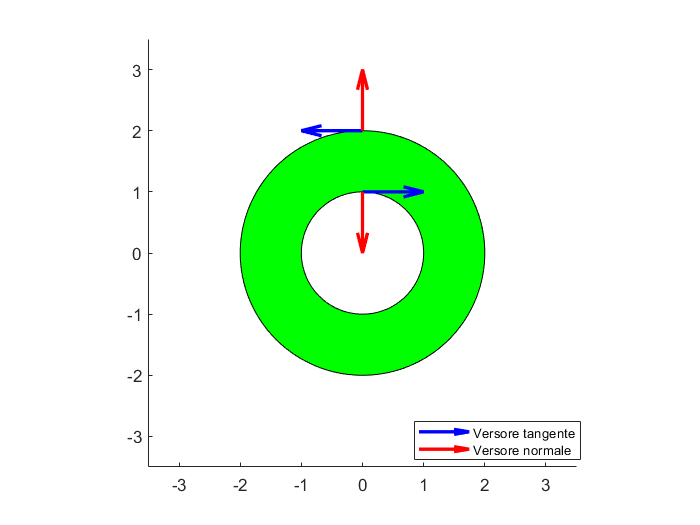
\includegraphics[width=\textwidth]{Capitoli/Capitolo5/Bordo orientato.png}
     \end{minipage}
     \begin{minipage}{0.4\textwidth}
         Affinché la frontiera della corona circolare sia orientata positivamente, occorre che la coppia di versori $N,\ T$ sia disposta come in figura. Da ciò si osserva che la circonferenza esterna deve essere percorsa in senso antiorario, quella interna nel senso opposto.
     \end{minipage}
 \end{figure}
 \begin{theorem}[Formule di Gauss-Green per domini regolari] \label{Teo: Formule di Gauss Green}
 Sia $f: D\subseteq \R^2 \to \R$ di classe $C^1(D)$. Se $D$ è un dominio normale regolare rispetto a $x$ si ha che
 \begin{equation} \label{Eq: Gauss-Green per dimostrazione}
     \iint\limits_D{\frac{\partial f}{\partial y}(x,y)}\,dx\,dy= -\int\limits_{\ppartial D}{f(x,y)}\,dx
 \end{equation}
     Se invece $D$ è un dominio normale regolare rispetto a $y$, vale
     \begin{equation}
    \iint\limits_D{\frac{\partial f}{\partial x}(x,y)}\,dx\,dy= \int\limits_{\ppartial D}{f(x,y)}\,dy
     \end{equation}
 \end{theorem}
 \begin{proof}
 Sia $D$ definito come segue:
        \begin{equation}
          D=  \left\{ (x,y) \in \R^2 \mid a \leq x \leq b,\ \alpha(x) \leq y \leq \beta(x)\right\}
        \end{equation}
Allora si ha che la frontiera di tale insieme può essere rappresentata come l'unione dei sostegni di quattro curve, come in figura.
 \begin{figure}[H]
     \centering
     \begin{minipage}{0.3\textwidth}
     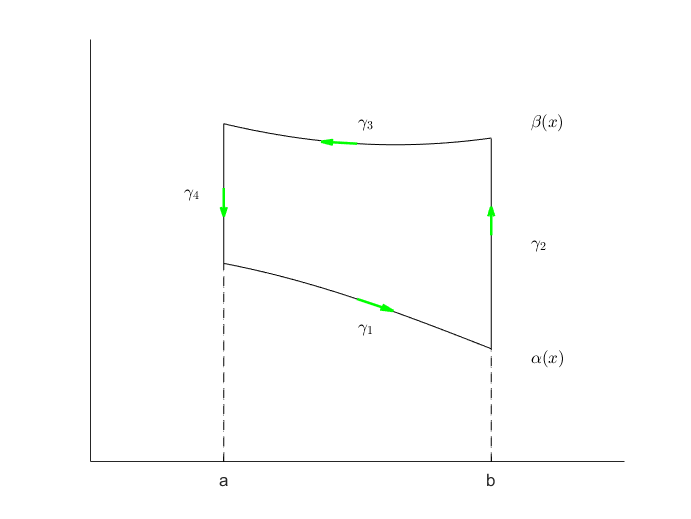
\includegraphics[width=\textwidth]{Capitoli/Capitolo5/Curve per GG.png}
     \end{minipage}
     \begin{minipage}{0.63\textwidth}
        Si parametrizzino i vari tratti di curva: 
        \begin{equation}
            \begin{aligned}
                &\gamma_1:\ \varphi_1(t)= \begin{cases}
                    t\\
                    \alpha(t)
                \end{cases}
                \quad t \in [a,b]\\
                &\gamma_2:\ \varphi_2(t)= \begin{cases}
                    b\\
                    t
                \end{cases}
                \quad t \in [\alpha(b), \beta(b)]\\
                &\gamma_3:\ \varphi_3(t)= \begin{cases}
                    a+b-t\\
                    \beta(a+b-t)
                \end{cases}
                \quad t \in [a,b]\\
                &\gamma_4: \varphi_4(t)= \begin{cases}
                    a\\
                    \beta(a)+\alpha(a)-t
                \end{cases}
                \quad t \in [\alpha(a), \beta(a)]
            \end{aligned}
        \end{equation}
     \end{minipage}
 \end{figure}
 \flushleft Dunque, si mostri, senza perdita di generalità, l'equivalenza degli integrali nella \eqref{Eq: Gauss-Green per dimostrazione}.
 \begin{equation}
    \begin{aligned}
     \iint\limits_D{\frac{\partial f}{\partial y}(x,y)}\,dx\,dy &\overset{\eqref{Eq: Formula di riduzione integrali doppi 1}}{=} \int\limits_{a}^{b}{\left( \int\limits_{\alpha(x)}^{\beta(x)}\frac{\partial f}{\partial y}(x,y)\,dy \right)}\, dx \overset{\text{TFC}}{=}\int\limits_{a}^{b}{ f(x, \beta(x))- f(x, \alpha(x))}\, dx
     \end{aligned}
 \end{equation}
Inoltre, 
\begin{equation}
\begin{aligned}
    \int\limits_{\ppartial D}{f}\, dx &= \sum\limits_{i=1}^{4} \int\limits_{\gamma_i}{f}\,dx =
    \int\limits_{a}^{b}{f(t, \alpha(t)) t'}\, dt+ \int\limits_{\alpha(b)}^{\beta(b)}{f(b,t)b'}\, dt +\\
    &+\int\limits_{a}^{b}{f(a+b-t, \beta(a+b-t))(a+b-t)'}\, dt + \int\limits_{\alpha(a)}^{\beta(a)}{f(a, \beta(a)+\alpha(a)-t) a'}\, dt=\\
    &= \int\limits_{a}^{b}{f(t, \alpha(t))}\, dt + \int\limits_{a}^{b}{-f(a+b-t, \beta(a+b-t))}\, dt =\\
    &\overset{\substack{\text{Nel }\#2:\\ a+b-t=s\\ -dt=ds}}{=} \int\limits_a^b{f(t, \alpha(t))}\, dt + \int\limits_a^b{f(s, \beta(s))}\, ds = \int\limits_{a}^{b}{f(t, \alpha(t))- f(t, \beta(t))}\, dt=\\
    &=-\int\limits_{a}^{b}{ f(t, \beta(t))- f(t, \alpha(t))}\, dt
    \end{aligned}
\end{equation}
Cioè la tesi.\\
Il ragionamento e la dimostrazione per la seconda parte della tesi sono analoghi.
 \end{proof}
 Dal teorema discende come corollario quanto segue.
 \begin{corollary}
     Sia $D$ un dominio normale regolare rispetto a entrambi gli assi e sia $\omega= P(x,y)dx+ Q(x,y)dy$ una forma differenziale di classe $C^1(D)$. Allora
     \begin{equation}
         \iint\limits_{D}{\left[\frac{\partial Q}{\partial x} (x,y)- \frac{\partial P}{\partial y}(x,y)\right]}\, dx\, dy = \int\limits_{\ppartial D} \omega
     \end{equation}
\end{corollary}
\begin{proof}
    La dimostrazione discende dall'applicazione del teorema precedente. Infatti,
    \begin{equation}
        \begin{aligned}
            &\iint\limits_{D}{\frac{\partial Q}{\partial x} (x,y)}\,dx\,dy =  \int\limits_{\ppartial D}{Q(x,y)}\,dy\\
            &\iint\limits_{D}{\frac{\partial P}{\partial y} (x,y)}\,dx\,dy =  -\int\limits_{\ppartial D}{P(x,y)}\,dx
        \end{aligned}
    \end{equation}
    Perciò, unendo tali risultati si ha che
    \begin{equation}
      \iint\limits_{D}{\left[\frac{\partial Q}{\partial x} (x,y)- \frac{\partial P}{\partial y}(x,y)\right]}\, dx\, dy = \int\limits_{\ppartial D}{Q(x,y)}\,dy - \left(  -\int\limits_{\ppartial D}{P(x,y)}\,dx\right)= \int\limits_{\ppartial D} \omega  
    \end{equation}
\end{proof}
\begin{oss}
A questo punto si può inoltre aggiungere che se $D$ è un dominio regolare qualsiasi definito come 
\begin{equation}
    D = \bigcup_{j=1}^{N} D_j
\end{equation}
allora continuano a valere le formule di Gauss-Green. Una dimostrazione di tale fatto si può avere sommando per additività gli integrali calcolati sui singoli tratti di frontiera. Infatti, laddove $\ppartial D_i$ e $\ppartial D_j$ coincidono, si ha che i versori normali hanno verso opposto e il loro contributo è nullo, lasciando come integrale risultante proprio
\begin{equation}
    \int\limits_{\ppartial D}{\omega}
\end{equation}
\end{oss}
Le formule di Gauss-Green possono essere utilizzate per il calcolo di aree racchiuse da curve. Infatti vale il seguente corollario.
\begin{corollary}[Gauss-Green per il calcolo di aree racchiuse da una curva]
Sia $D \subseteq \R^2$ un dominio regolare. Allora,
\begin{equation}
    \area(D)= \int\limits_{\ppartial D}{x}\, dy = -\int\limits_{\ppartial D}{y}\, dx = \frac{1}{\alpha+\beta}{\int\limits_{\ppartial D}{\alpha x dy - \beta y dx}} \qquad \forall\ \alpha, \beta \in \R,\ \alpha+\beta \neq 0
\end{equation}
\end{corollary}
\begin{proof}
    Per definizione 
    \begin{equation}
        \area(D)= \iint\limits_{D}{1}\,dx\, dy
    \end{equation}
    Allora si ha che
    \begin{align}
        &1= \frac{\partial f}{\partial y} \Rightarrow f(x,y)= y \Rightarrow \area(D)= \iint\limits_{D} \frac{\partial f}{\partial y} \overset{\text{G.G.}}{=}  -\int\limits_{\ppartial D}{y}\,dx\\
      &  1=\frac{\partial f}{\partial x} \Rightarrow f(x,y)= x \Rightarrow \area(D)= \iint\limits_{D} \frac{\partial f}{\partial x} \overset{\text{G.G.}}{=}  \int\limits_{\ppartial D}{x}\,dy
    \end{align}
    Perciò, si ha che
    \begin{equation}
        (\alpha+\beta)\area(D)= \int\limits_{\ppartial D}{\alpha x dy - \beta y dx} \Rightarrow \area(D)=  \frac{1}{\alpha+\beta}{\int\limits_{\ppartial D}{\alpha x dy - \beta y dx}}
    \end{equation}
\end{proof}